\chapter{Optimalisatie}
\label{opt}

\begin{figure}[h!]
\centering
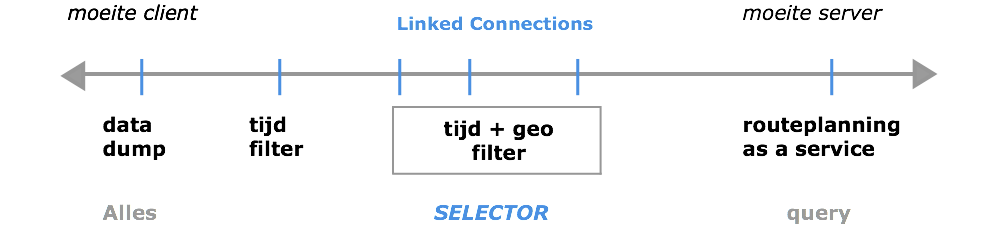
\includegraphics[scale=0.4]{LDF-as4.png}
\caption{Linked Data Fragmenten-as met Linked Connections optimalisatietechniek}
\end{figure}

\section{Geofiltering}

\section{Server}

\subsection{Cachebaarheid}

Aantal mogelijke URI's voor 1 dag met enkel tijdsfilter en fragmenten om de 10 minuten:
24u * 60 min / 10 min = 144 URI's
\subsection{Grootte fragmenten}

Hoeveel connecties per fragment best?
Hangt samen met snelheid
Snelheid requests < snelheid verwerken connecties ? Is er bottleneck?

Verhouding aantal connecties/request -> tijdsinterval aanpassen

\subsection{Burenconnecties}

\section{Client}

\subsection{Heuristiek}

\begin{figure}[h!]
\centering
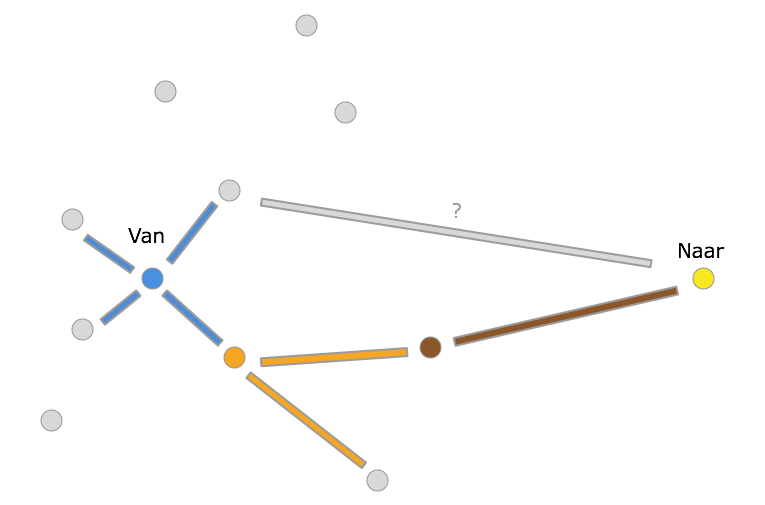
\includegraphics[scale=0.5]{HeuristiekClient.png}
\caption{Heuristiek client voor volgende vertrekstop}
\end{figure}


\section{Voor- en nadelen}